\documentclass[english, a4paper, 11pt]{article}


%%%%%%%%%%% LANGUAGE %%%%%%%%%%%

% For correct hyphenation in swedish
\usepackage[T1]{fontenc}

% For interpreting non-ASCII characters
% \usepackage[utf8]{inputenc}

% International language support
% Fetches language from documentclass options. Most other packages do this as well
\usepackage{babel}


%%%%%%%%%%% FORMAL STUFF %%%%%%%%%%%

% Smaller margins
\usepackage[margin=2.5cm]{geometry}

% Clickable urls
\usepackage[hyphens]{url} % Does not want to be loaded after physics package

% Fancy chapter headers
\usepackage{titlesec}
\titleformat{\chapter}{\normalfont\huge}{\thechapter.}{20pt}{\huge\it}

% Dates & time
\usepackage{datetime} % Useful when referencing websites

% What to display in table of contents
\setcounter{tocdepth}{3}
\setcounter{secnumdepth}{3}

% Lists
\usepackage{enumerate} % Determines the style in which the counter is printed
\usepackage{enumitem} % Provides user control over the layout of the three basic list environments

% Citing & bibliography
\usepackage{csquotes} % For \enquote command for proper quotation marks, also biblatex recommends this
\usepackage[backend=biber, style=numeric, sorting=none]{biblatex}
\bibliography{bibliography} % A file named bibliography.bib containing the bibTeX entries should be placed beside the main.tex file


%%%%%%%%%%% GRAPHICS %%%%%%%%%%%

\usepackage{graphics,color,xcolor}

% Figures
\usepackage{epsfig} % Solves some problems in \includegraphics{<.eps-file>}
\usepackage{graphicx} % More options for \includegraphics
\usepackage{wrapfig} % Figure environment that lets text wrap around figure
\usepackage{float} % Figure placement
\usepackage{caption} % More options for \caption
\usepackage{subcaption} % Subfigures

% Tikz
\usepackage{tikz}
\usepackage{pgf,pgfplots} % Pgfplot
\pgfplotsset{compat=1.15}

% För alduslöv
\usepackage{pifont}


%%%%%%%%%%% PHYSICS %%%%%%%%%%%

% SI units
\usepackage{siunitx}

% Physics macros
\usepackage{physics} % Defines lots of nice commands like \derivative, \norm, \evaluated, etc. It is recommended to use these as much as possible for nice spacing and readable LaTeX code.
\usepackage{braket} % Defines \bra, \ket, \braket, and \set
\usepackage{cancel} % Basically a better version of the \not command
\usepackage{slashed} % For Feynman slash notation
\usepackage{simpler-wick} % Wick contractions (may require sty-file)
\usepackage[compat=1.1.0]{tikz-feynman} % Feynman diagrams (has to be compiled with LuaTeX)


%%%%%%%%%%% CODING %%%%%%%%%%%

% For nice code insertions
\usepackage{listings}
\definecolor{codegreen}{rgb}{0,0.6,0}
\definecolor{codegray}{rgb}{0.5,0.5,0.5}
\definecolor{codepurple}{rgb}{0.58,0,0.82}
\definecolor{backcolour}{rgb}{0.95,0.95,0.92}
\lstdefinestyle{mystyle}{
    backgroundcolor=\color{backcolour},   
    commentstyle=\color{codegreen},
    keywordstyle=\color{magenta},
    numberstyle=\tiny\color{codegray},
    stringstyle=\color{codepurple},
    basicstyle=\ttfamily\footnotesize,
    breakatwhitespace=false,         
    breaklines=true,                 
    captionpos=b,                    
    keepspaces=true,                 
    numbers=left,                    
    numbersep=5pt,                  
    showspaces=false,                
    showstringspaces=false,
    showtabs=false,                  
    tabsize=2
}
\lstset{style=mystyle}


%%%%%%%%%%% MATHEMATICS %%%%%%%%%%%

% AMS packages
\usepackage{amsmath,amsfonts,amsthm,amssymb}

% Sats/bevismiljöer
\iflanguage{swedish}{
    \newtheorem{theorem}{Sats}
    \newtheorem*{theorem*}{Sats}
    \newtheorem{lemma}{Lemma}
    \newtheorem*{lemma*}{Lemma}
    \renewenvironment{proof}{\textit{Bevis.}}{\hfill$\square$}
    \theoremstyle{definition}
    \newtheorem{definition}{Definition}
    \newtheorem*{definition*}{Definition}
}{}
\iflanguage{english}{
    \newtheorem{theorem}{Theorem}
    \newtheorem*{theorem*}{Theorem}
    \newtheorem{lemma}{Lemma}
    \newtheorem*{lemma*}{Lemma}
    \renewenvironment{proof}{\textit{Proof.}}{\hfill$\square$}
    \theoremstyle{definition}
    \newtheorem{definition}{Definition}
    \newtheorem*{definition*}{Definition}
}{}

% Vectors are upright boldface. This definition is better than the physics package's \vectorbold I think.
\renewcommand{\Vec}[1]{{\boldsymbol{\mathrm{#1}}}}
\renewcommand{\vec}[1]{{\boldsymbol{\mathrm{#1}}}}

% Redefine \exp
% Errors occur if this definition is made before some of the packages are loaded
\let\oldexp\exp
\newcommand{\Exp}[1]{\oldexp{#1}}
\renewcommand{\exp}[1]{\mathrm{e}^{#1}}

% Some of my own shorthands for correct spacing in math environments
\newcommand{\from}{\colon} % Proper spacing of colon in functions f: A → B


%%%%%%%%%%% MISCELLANEOUS %%%%%%%%%%%

% In-pdf comments through \todo command
\setlength{\marginparwidth}{2cm} % Silence warning about margin size
\usepackage{todonotes}

% Clickable links and refs
\usepackage[hidelinks]{hyperref} 

% Cleverref automatically detects if you are referencing a figure, table, or equation etc
% Cleverref has to be loaded last I think, after babel and hyperref etc
\usepackage[noabbrev, nameinlink]{cleveref}
\crefname{equation}{}{}
\iflanguage{swedish}{ % Tell cleverref to use Oxford comma
	\newcommand{\creflastconjunction}{, och\nobreakspace}
}{}
\iflanguage{english}{
	\newcommand{\creflastconjunction}{, and\nobreakspace}
}{}


% Tag only referenced equations (this is not an ideal package, as it requires etextools, which is buggy and abandoned by its author)
% \expandafter\def\csname ver@etex.sty\endcsname{3000/12/31}
% \let\globcount\newcount
% \usepackage{autonum}

% For writing \overset{text}&{=} in align environment
\usepackage{aligned-overset} 

% number sections by a), b), etc & subsections by (i), (ii), etc
\renewcommand{\thesection}{\alph{section})}
\renewcommand{\thesubsection}{\alph{section}.\roman{subsection})}

% Bar and tilde that scales with what is under them. Basically I just want these to have consistent names
\newcommand{\mathbar}[1]{\overline{#1}}
\newcommand{\mathtilde}[1]{\widetilde{#1}}
\newcommand{\mathhat}[1]{\widehat{#1}}


\title{{\Huge \ding{166}} Quantum Field Theory Problem 6 {\Huge \ding{166}}}
\author{simjac}
\date{\monthname[\the\month] 2020}

\begin{document}

\maketitle

Consider the pseudoscalar Yukawa Lagrangian,
\begin{align}\label{eq:pseduoscalar_yukawa_lagrangian}
    \mathcal{L}_\mathrm{Yukawa} = \frac{1}{2} (\partial_\mu \phi)^2 - \frac{1}{2} m_\phi^2 \phi^2 - \mathbar{\psi} (i \slashed{\partial} - m_\psi) \psi - i g \mathbar{\psi} \gamma^5 \psi \phi,
\end{align}
where $\phi$ is a real scalar field and $\psi$ is a Dirac fermion. Notice that this Lagrangian is invariant under the parity transform \begin{align}
	\psi(t, \Vec{x}) \mapsto \gamma^0 \psi(t, -\Vec{x}) \label{eq:psi_parity_transformation}\\
	\phi(t, \Vec{x}) \mapsto -\phi(t, -\Vec{x}) \label{eq:phi_parity_transformation}
\end{align}
in which the field $\phi$ carries odd parity.

\section{}

\subsection{}
Determine the superficially divergent amplitude.

\subsection*{Solution}
We have the interaction Hamiltonian
\begin{align}
	\mathcal{H}_\mathrm{I} = i g \mathbar{\psi} \gamma^5 \psi \phi
\end{align}
We want to calculate the two-point correlation function
\begin{align}
	\bra{\Omega} T \phi(x) \phi(y) \ket{\Omega} = \bra{0} T \left\{ \phi_\mathrm{I}(x) \phi_\mathrm{I}(y) \Exp{-i \int^T_{-T} \dd{t} H_\mathrm{I}(t)} \right\} \Ket{0}
\end{align}
The non-zero Feynman rules for the pseudoscalar Yukawa theory are
\begin{align}
	\feynmandiagram[small, inline=(o.base), horizontal=a to o]{
		a [particle=$\phi$]-- [scalar] o [particle=$\phi$],
	};
	&= \frac{i}{p^2 - m_\phi^2} \label{eq:phi_to_phi_feynman_rule}\\
	\feynmandiagram[small, inline=(o.base), horizontal=a to o]{
		a [particle=$\psi$] -- [fermion] o [particle=$\mathbar{\psi}$],
	};
	&= \frac{i (\slashed{p} + m_\psi)}{p^2 - m_\psi^2} \label{eq:psi_to_psibar_feynman_rule}\\
	\feynmandiagram[small, inline=(o.base), horizontal=o to a]{
		o [dot],
		o -- [scalar] a,
		o -- [fermion] b,
		c -- [fermion] o,
	};
	&= g \gamma^5.\label{eq:phi_psi_psibar_vertex_feynman_rule}
\end{align}

Consider, similarly to what Peskin does on page 316, a general Feynman diagram in this theory. Define
\begin{align*}
	N_\phi &= \textrm{\# of external $\phi$ lines}\\
	N_\psi &= \textrm{\# of external $\psi$ lines}\\
	P_\phi &= \textrm{\# of $\phi$ propagators}\\
	P_\psi &= \textrm{\# of $\psi$ propagators}\\
	V &= \textrm{\# of vertices}\\
	L &= \textrm{\# of loops}.
\end{align*}
The expression corresponding to a general diagram would then be proportianal to
\begin{align}
	g^V \int
	\frac{\dd[4]{p_1} \cdots \dd[4]{p_{P_\phi}}}{(p_1^2 - m_\phi^2) \cdots (p_{P_\phi}^2 - m_\phi^2)}
	\frac{(\slashed{p}_1 + m_\psi) \dd[4]{q_1} \cdots (\slashed{p}_{P_\phi} + m_\psi) \dd[4]{q_{P_\psi}}}{(q_1^2 - m_\psi^2) \cdots (p_{P_\psi}^2 - m_\psi^2)}.
\end{align}
Counting powers of momenta in this integral gives us the superficial degree of divergence
\begin{align}
	D = 4 L - P_\psi - 2 P_\phi.
\end{align}
Using Euler's formula for planar graphs ($L = P_\phi + P_\psi - V + 1$) and $V = 2 P_\psi + N_\psi = P_\phi + \frac{1}{2} N_\phi$ (since \cref{eq:phi_psi_psibar_vertex_feynman_rule} is the only nonzero vertex, we are guaranteed that there are two $\psi$ and one $\phi$ propagator per vertex), we rewrite this as
\begin{align}
	D = 4 - N_\phi - \frac{3}{2} N_\psi.
\end{align}
There are seven configurations satisfying $D \geq 0$ and hence there are seven superficially divergent Feynman diagrams. These diagrams are shown in \cref{fig:superficially_divergent_diagrams}.

\begin{figure}[H]
    \centering
    \begin{subfigure}{.33\linewidth}
        \centering
        \feynmandiagram[small, inline=(o.base), vertical=a to o]{
        	o [blob],
        	i1 -- [draw=none] o,
            i2 -- [draw=none] o,
            i3 -- [draw=none] o,
            i4 -- [draw=none] o,
        };
        \caption{$D = 4$}
        \label{subfig:superficially_divergent_diagrams:a}
    \end{subfigure}%
    \begin{subfigure}{.33\linewidth}
        \centering
        \feynmandiagram[small, inline=(o.base), horizontal=o to a]{
        	o [blob],
        	a -- [scalar] o,
        	i1 -- [draw=none] o,
            i2 -- [draw=none] o,
            i3 -- [draw=none] o,
        };
        \caption{$D = 3$}
        \label{subfig:superficially_divergent_diagrams:b}
    \end{subfigure}%
    \begin{subfigure}{.33\linewidth}
        \centering
        \feynmandiagram[small, inline=(o.base), horizontal=a to o]{
        	o [blob],
        	i1 -- [draw=none] o,
        	i2 -- [draw=none] o,
            a -- [scalar] o,
            b -- [scalar] o,
        };
        \caption{$D = 2$}
        \label{subfig:superficially_divergent_diagrams:c}
    \end{subfigure}
    \begin{subfigure}{.33\linewidth}
        \centering
        \feynmandiagram[small, inline=(o.base), horizontal=o to a]{
        	o [blob],
        	a -- [scalar] o,
        	b -- [scalar] o,
            c -- [scalar] o,
        };
        \caption{$D = 1$}
        \label{subfig:superficially_divergent_diagrams:d}
    \end{subfigure}%
    \begin{subfigure}{.33\linewidth}
        \centering
        \feynmandiagram[small, inline=(o.base), vertical=a to b]{
        	o [blob],
        	a -- [scalar] o,
        	b -- [scalar] o,
        	a -- [draw=none] b,
            c -- [scalar] o,
            d -- [scalar] o,
        	c -- [draw=none] d,
        };
        \caption{$D = 0$}
        \label{subfig:superficially_divergent_diagrams:e}
    \end{subfigure}%
    \begin{subfigure}{.33\linewidth}
        \centering
        \feynmandiagram[small, inline=(o.base), horizontal=a to o]{
        	o [blob],
        	i1 -- [draw=none] o,
        	i2 -- [draw=none] o,
            o -- [fermion] a,
            b -- [fermion] o,
        };
        \caption{$D = 1$}
        \label{subfig:superficially_divergent_diagrams:f}
    \end{subfigure}
    \begin{subfigure}{.33\linewidth}
        \centering
        \feynmandiagram[small, inline=(o.base), vertical=a to o]{
        	o [blob],
            a -- [scalar] o,
            o -- [fermion] b,
            c -- [fermion] o,
        };
        \caption{$D = 0$}
        \label{subfig:superficially_divergent_diagrams:g}
    \end{subfigure}
    \caption{
%    We can translate the diagrams in figure 10.2 in Peskin to the pseduoscalar Yukawa theory by changing the photon propagators to scalar propagators. We have also added the arrows that are not written out in figure 10.2 (the directions of these arrows follow from momentum conservation TODO: DO I KNOW THIS IS TRUE?).
	}
    \label{fig:superficially_divergent_diagrams}
\end{figure}


The first diagram, \cref{subfig:superficially_divergent_diagrams:a}, will add an infinite contribution to the vacuum energy. This will not be measurable. By \cref{eq:phi_parity_transformation}, any diagram with an odd number of external $\phi$-legs will be zero for symmetry reasons. Thus \cref{subfig:superficially_divergent_diagrams:b} and \cref{subfig:superficially_divergent_diagrams:d} are zero.

Since we are only interested in one-loop diagrams, and there is only one type of vertex, there is only one type of diagram that we are interested in for each Feynman diagram in \cref{fig:superficially_divergent_diagrams}. These are shown in \cref{fig:one-loop_diagrams}.
\begin{figure}[H]
    \centering
    \begin{subfigure}{.33\linewidth}
		\centering
		\feynmandiagram[small, inline=(o1.base), horizontal=a to b]{
			a -- [scalar] o1,
			o1 -- [fermion, half left] o2,
			o2 -- [fermion, half left] o1,
			b -- [scalar] o2,
		};
		\setcounter{subfigure}{2}
		\caption{}
		\label{subfig:one-loop_diagrams:c}
	\end{subfigure}%
    \begin{subfigure}{.33\linewidth}
        \centering
        \feynmandiagram[small, inline=(o1.base), horizontal=o1 to o2]{
			a -- [scalar] o1,
			o1 -- [fermion, quarter right] o2,
			b -- [scalar] o2,
			o2 -- [fermion, quarter right] o3,
			c -- [scalar] o3,
			o3 -- [fermion, quarter right] o4,
			d -- [scalar] o4,
			o4 -- [fermion, quarter right] o1,
        };
		\setcounter{subfigure}{4}
        \caption{}
        \label{subfig:one-loop_diagrams:e}
    \end{subfigure}%
    \begin{subfigure}{.33\linewidth}
        \centering
        \feynmandiagram[small, inline=(o1.base), horizontal=a to b]{
            a -- [fermion] o1,
			o1 -- [fermion, half left] o2,
			o2 -- [scalar, half left] o1,
			o2 -- [fermion] b,
        };
        \caption{}
        \label{subfig:one-loop_diagrams:f}
    \end{subfigure}
    \begin{subfigure}{.33\linewidth}
        \centering
        \feynmandiagram[small, inline=(o.base), horizontal=o2 to o3]{
			a -- [fermion] o1,
			o1 -- [fermion, quarter right] o2,
			b -- [scalar] o2,
			o2 -- [fermion, quarter right] o3,
			o3 -- [fermion] c,
			o3 -- [scalar, quarter right] o1,
        };
        \caption{}
        \label{subfig:one-loop_diagrams:g}
    \end{subfigure}
    \caption{}
    \label{fig:one-loop_diagrams}
\end{figure}
These have the following divergences (compare with Peskin section 10.1):
\begin{align}
	&\textrm{\cref{subfig:one-loop_diagrams:c} $\propto a_0 \Lambda^2 + a_1 p^2 \log{\Lambda}$}\\
	%
	&\textrm{\cref{subfig:one-loop_diagrams:e} $\propto \log{\Lambda}$} \label{eq:superficially_divergent_phi^4}\\
	%
	&\textrm{\cref{subfig:one-loop_diagrams:f} $\propto a_0 \Lambda + \slashed{p} \log{\Lambda}$}\\
	%
	&\textrm{\cref{subfig:one-loop_diagrams:g} $\propto \log{\Lambda}$.}
\end{align}





\subsection{}
Work out the Feynman rules for renormalized perturbation theory for this Lagrangian. Include all necessary counterterm vertices.

\subsection*{Solution}
We follow Peskin section 10.2. Since \cref{subfig:one-loop_diagrams:e} is divergent, but \cref{eq:pseduoscalar_yukawa_lagrangian} contains no $\phi^4$-term, we see that we will have to add such a counterterm
\begin{align}\label{eq:phi^4-term}
	\frac{\lambda}{4!} \phi^4.
\end{align}
Define the renormalized fields $\phi_r$ and $\psi_r$ by
\begin{align}
	\phi &= Z_\phi^\frac{1}{2} \phi_r \label{eq:phi_renormalized}\\
	\psi &= Z_\psi^\frac{1}{2} \psi_r \label{eq:psi_renormalized}.
\end{align}
Putting \cref{eq:phi^4-term,,eq:phi_renormalized,,eq:psi_renormalized} into \cref{eq:pseduoscalar_yukawa_lagrangian}, we get
\begin{align}
	\mathcal{L} = \frac{1}{2} Z_\phi (\partial_\mu \phi_r)^2 - \frac{1}{2} Z_\phi m_\phi^2 \phi_r^2 + Z_\psi \mathbar{\psi}_r (i \slashed{\partial} - m_\psi) \psi_r - i Z_\psi Z_\phi^\frac{1}{2} g ̄\mathbar{\psi}_r \gamma^5 \psi_r \phi_r - \frac{\lambda}{4!}Z_\phi^2 \phi_r^4.
\end{align}
Defining
\begin{align*}
	\delta_{m_\phi} &= Z_\phi m_\phi^2 - m_{\phi_r}^2\\
	%
	\delta_{m_\psi} &= Z_\psi m_{\psi} - m_{\psi_r}\\
	%
	\delta_{Z_\phi} &= Z_\phi - 1\\
	%
	\delta_{\lambda} &= \lambda Z_\phi^2 - \lambda_r\\
	%
	\delta_{g} &= \frac{g}{g_r} Z_\psi Z_\phi^\frac{1}{2} - 1\\
	%
	\delta_{Z_\psi} &= Z_\psi - 1,
\end{align*}
where the variables with an $r$-index will correspond to observables. This gives us the renormalized Lagrangian on the form
\begin{align*}
	\mathcal{L} &= \dfrac{1}{2}(\partial_\mu \phi_r)^2 - \frac{1}{2} m_{\phi_r}^2 \phi_r^2 + \mathbar{\psi}_r (i \slashed{\partial} - m_{\psi_r}) \psi_r - i g_r \mathbar{\psi}_r \gamma^5 \psi_r \phi_r - \frac{\lambda}{4!} \phi_r^4\\
	%
	&+ \frac{1}{2} \delta_{Z_\phi} (\partial_\mu \phi_r)^2 - \frac{1}{2} \delta_{m_\phi} m_{\phi_r}^2 \phi_r^2 + \mathbar{\psi}_r (i \delta_{Z_\psi} \slashed{\partial} - \delta_{m_\psi} ) \psi_r - i g_r \delta_g \mathbar{\psi}_r \gamma^5 \psi_r \phi_r - \frac{\delta_\lambda}{4!} \phi_r^4.
\end{align*}
The second line here are all the counterterms. Reading off their Feynman rules from the Lagrangian (the symmetry factors from Peskin page 93 determine the overall constant), we have 
\begin{align}
	\feynmandiagram[small, inline=(o.base), horizontal=a to o]{
		a [particle=$\phi$]-- [scalar] o [particle=$\phi$],
	};
	&= \frac{i}{p^2 - m_{\phi_r}^2} \label{eq:renormalized_phi_to_phi_feynman_rule}\\
	%
	\feynmandiagram[small, inline=(o.base), horizontal=a to o]{
		a [particle=$\psi$] -- [fermion] o [particle=$\mathbar{\psi}$],
	};
	&= \frac{i (\slashed{p} + m_{\psi_r})}{p^2 - m_{\psi_r}^2} \label{eq:renormalized_psi_to_psibar_feynman_rule}\\
	%
	\feynmandiagram[small, inline=(o.base), horizontal=o to a]{
		o [dot],
		o -- [scalar] a,
		o -- [fermion] b,
		c -- [fermion] o,
	};
	&= g_r \gamma^5
	\label{eq:renormalized_phi_psi_psibar_vertex_feynman_rule}\\
	%
	\feynmandiagram[small, inline=(o.base), vertical=a to b]{
		o [dot],
		a [particle=$\phi$] -- [scalar] o,
		b [particle=$\phi$] -- [scalar] o,
		c [particle=$\phi$] -- [scalar] o,
		d [particle=$\phi$] -- [scalar] o,
		a -- [draw=none] b,
		c -- [draw=none] d,
	};
	&= -i \lambda_r
	\label{eq:renormalized_phi^4_vertex_feynman_rule}\\
	%
	\feynmandiagram[small, inline=(o.base), horizontal=a to o]{
		o [crossed dot],
		a [particle=$\phi$] -- [scalar] o,
		o -- [scalar] b [particle=$\phi$],
	};
	&= i (p^2 \delta_{Z_\phi} - \delta_{m_\phi})\\
	%
	\feynmandiagram[small, inline=(o.base), horizontal=a to o]{
		o [crossed dot],
		a [particle=$\psi$] -- [fermion] o,
		o -- [fermion] b [particle=$\mathbar{\psi}$],
	};
	&= i (\slashed{p} \delta_{Z_\psi} - \delta_{m_\psi})
	\label{eq:renormalized_counterterm_phi_phi_feynman_rule}\\
	%
	\feynmandiagram[small, inline=(o.base), vertical=a to b]{
		o [crossed dot],
		a [particle=$\phi$] -- [scalar] o,
		b [particle=$\phi$] -- [scalar] o,
		c [particle=$\phi$] -- [scalar] o,
		d [particle=$\phi$] -- [scalar] o,
		a -- [draw=none] b,
		c -- [draw=none] d,
	};
	&= -i \delta_\lambda\\
	%
	\feynmandiagram[small, inline=(o.base), horizontal=o to a]{
		o [crossed dot],
		o -- [scalar] a,
		o -- [fermion] b,
		c -- [fermion] o,
	};
	&= g_r \delta_{g} \gamma^5 \label{eq:renormalized_counterterm_psi_psibar_phi_vertex_feynman_rule}
\end{align}

The diagrams with an $\otimes$ are the counterterms. We see that \cref{eq:renormalized_phi_to_phi_feynman_rule,,eq:renormalized_psi_to_psibar_feynman_rule,,eq:renormalized_phi_psi_psibar_vertex_feynman_rule} are basically the same as \cref{eq:phi_to_phi_feynman_rule,,eq:psi_to_psibar_feynman_rule,,eq:phi_psi_psibar_vertex_feynman_rule} but with the renormalized fields instead.







\subsection{}
Show that the theory contains a superficially divergent $4 \phi$ amplitude.

\subsection*{Solution}

This is what \cref{eq:superficially_divergent_phi^4} states.




\subsection{}
This means that the theory cannot be renormalized unless one includes a scalar self-interaction
\begin{align}
    \delta \mathcal{L} = \frac{\lambda}{4!} \phi^4,
\end{align}
and a counterterm of the same form. It is of course possible to set the renormalized value of this coupling to zero, but that is not a natural choice, since the counterterm will still be nonzero. Are any further interactions required.

\subsection*{Solution}

No, I don't think so.


\section{}

Compute the divergent part (the pole as $d \to 4$) of each counterterm, to the one-loop order of perturbation theory, implementing a sufficient set of renormalization conditions. You need not worry about finite parts of the counterterms. Since the divergent parts must have a fixed dependence on the external momenta, you can simplify this calculation by choosing the momenta in the simplest possible way.

\subsection*{Solution}
Now that we have one more vertex allowed, \cref{eq:renormalized_phi^4_vertex_feynman_rule}, there is no longer just one one-loop diagram corresponding to each diagram in \cref{fig:superficially_divergent_diagrams}. For example, we have that
\begin{align}\label{eq:c_renormalized}
	\feynmandiagram[small, inline=(o.base), horizontal=a to o]{
		o [blob],
		a -- [scalar] o,
		b -- [scalar] o,
	};
	&=
	\feynmandiagram[small, inline=(o1.base), horizontal=a to b]{
		a -- [scalar] o1,
		o1 -- [fermion, half left] o2,
		o2 -- [fermion, half left] o1,
		b -- [scalar] o2,
	};
	+
	\feynmandiagram[small, inline=(o1.base), horizontal=a to b]{
		o [dot],
		o -- [scalar, out=135, in=45, loop, min distance=2cm] o,
		a -- [scalar] o,
		o -- [scalar] b,
	};
	+
	\feynmandiagram[small, inline=(o1.base), horizontal=a to b]{
		o [crossed dot],
		a -- [scalar] o,
		o -- [scalar] b,
	};
	+	\feynmandiagram[small, inline=(o1.base), horizontal=a to b]{
		a -- [scalar] b,
	};
	.
\end{align}
We may impose, as Peskin does in (10.19), the renormalization conditions 
\begin{align}
	\feynmandiagram[small, inline=(o.base), horizontal=a to o]{
		o [blob],
		a -- [scalar] o,
		b -- [scalar] o,
	};
	&= \frac{i}{p^2 - m_{\phi_r}^2}
	\label{eq:phi_phi_renormalization_condition}\\
	%
    \feynmandiagram[small, inline=(o.base), vertical=a to b]{
		o [blob],
		a -- [scalar] o,
		b -- [scalar] o,
		a -- [draw=none] b,
		c -- [scalar] o,
		d -- [scalar] o,
		c -- [draw=none] d,
	};
	&= -i \lambda_r \quad \textrm{at } s = 4 m^2, t = u = 0
	\label{eq:phi^4_renormalization_condition}\\
	%
	\feynmandiagram[small, inline=(o.base), horizontal=a to o]{
		o [blob],
		a -- [fermion] o,
		o -- [fermion] b,
	};
	&= \frac{i}{\slashed{p} - m_{\psi_r}}
	\label{eq:psi_psibar_renormalization_condition}\\
	%
	\feynmandiagram[small, inline=(o.base), horizontal=o to a]{
		o [blob],
		o -- [scalar] a,
		o -- [fermion] b,
		c -- [fermion] o,
	};
	&= g_r \gamma^5
	\label{eq:phi_psi_psibar_renormalization_condition}\\
\end{align}
and, as Peskin does in (10.28) and (10.40), state that this is equivalent to
\begin{align}
	M^2(p^2) \eval_{p^2 = m_{\phi_r}^2} &= 0\\
	%
	\Sigma(\slashed{p}) \eval_{\slashed{p} = m_{\psi_r}} &= 0\\
	%
	\derivative{}{p^2} M^2(p^2) \eval_{p^2 = m_{\phi_r}^2} &= 0\\
	%
	\derivative{}{p^2} \Sigma(\slashed{p}) \eval_{\slashed{p} = m_{\psi_r}} &= 0.
\end{align}
Considering only the divergent terms of \cref{eq:c_renormalized}, we have (as on page 328--329 in Peskin)
\begin{align}
	\feynmandiagram[small, inline=(o1.base), horizontal=a to b]{
		a -- [scalar] o1,
		o1 -- [fermion, half left] o2,
		o2 -- [fermion, half left] o1,
		b -- [scalar] o2,
	};
	\overset{\textrm{\cref{eq:renormalized_psi_to_psibar_feynman_rule,eq:renormalized_phi_psi_psibar_vertex_feynman_rule}}}&{=} (-i g_r)^2 \int \frac{\dd[d]{k}}{(2 \pi)^d} \tr{\frac{i}{\slashed{k} - m_{\psi_r}} \gamma^5 \frac{i}{(\slashed{k} - \slashed{p}) - m_{\psi_r}} \gamma^5} \notag\\
	%
	\overset{\textrm{\cref{fig:trace_calculation}}}&{=} (-i g_r)^2 \int \frac{\dd[d]{k}}{(2 \pi)^d} \frac{4 \left( k \cdot (k + p) - m_{\psi_r}^2 \right)}{(k^2 - m_{\psi_r}^2) \left( (k + p)^2 - m_{\psi_r}^2 \right)} \notag\\
	%
	&\left\{ \frac{1}{A B} = \int_0^1 \dd{x} \frac{1}{ \left(x A - (1 - x) B \right)^2} \right\} \notag\\
	%
	&= 4 (-i g_r)^2 \int_0^1 \dd{x} \int \frac{\dd[d]{k}}{(2 \pi)^d} \frac{k \cdot (k + p) - m_{\psi_r}^2}{x (k + p)^2 - x m_{\psi_r}^2 + k^2 - m_{\psi_r}^2 - x k^2 + x m_{\psi_r}^2} \notag\\
	%
	&\left\{ \textrm{define } \quad
		\begin{matrix}
			\ell = k + x p\\
			\Delta = -x (1 - x) p^2 + m_{\psi_r}^2
		\end{matrix}
	\right\} \notag\\
	%
	&= 4 (-i g_r)^2 \int \frac{\dd[d]{\ell}}{(2 \pi)^d} \int_0^1 \dd{x} \frac{\ell^2 - x (1 - x) p^2 - m_{\psi_r}^2}{(\ell^2 - \Delta)^2} \notag\\
	%
	\overset{\textrm{Peskin (A.44) and (A.45)}}&{=} 4 (-i g_r)^2 \int_0^1 \dd{x} \frac{1}{(4 \pi)^\frac{d}{2}} \left[ -\frac{d \Gamma(2 - \frac{d}{2})}{\Delta^{2 - \frac{d}{2}}} - \frac{d \Gamma(2 - \frac{d}{2})}{\Delta^{2 - \frac{d}{2}}} \left( x (1 - x) p^2 + m_{\psi_r}^2 \right) \right]\notag\\
	%
	\overset{\textrm{Peskin (A.49) and (A-50)}}&{=} \frac{-i g_r^2 (m_{\psi_r}^2 - \frac{1}{2} p^2)}{2 \pi^2 (d - 4)} + \mathcal{O}\left( (d - 4)^0 \right). \label{eq:first_term_in_phi_phi_diagram_calculated}
\end{align}
\begin{align}
	\feynmandiagram[small, inline=(o1.base), horizontal=a to b]{
		o [dot],
		o -- [scalar, out=135, in=45, loop, min distance=2cm] o,
		a -- [scalar] o,
		o -- [scalar] b,
	};
	\overset{\textrm{\cref{eq:renormalized_phi^4_vertex_feynman_rule,eq:renormalized_phi_to_phi_feynman_rule}}}&{=} -i \lambda_r \frac{1}{2} \int \frac{\dd[d]{k}}{(2 \pi)^d} \frac{i}{k^2 - m_{\phi_r}^2} \notag\\
	%
	\overset{\textrm{(A.44) in Peskin}}&{=} - i \lambda_r \frac{1}{(4 \pi)^\frac{d}{2} m_{\phi_r}^{2 - d}} \Gamma \left( 1 - \frac{d}{2} \right) \notag\\
	%
	\overset{\textrm{(A.50) in Peskin}}&{=} -i \lambda_r \frac{m_{\phi_r}^2}{16 \pi^2 (d - 4)} + \mathcal{O}\left( (d - 4)^0 \right) \label{eq:second_term_in_phi_phi_diagram_calculated}
\end{align}
\begin{align}
		\feynmandiagram[small, inline=(o1.base), horizontal=a to b]{
		o [crossed dot],
		a -- [scalar] o,
		o -- [scalar] b,
	};
	\overset{\textrm{\cref{eq:renormalized_counterterm_phi_phi_feynman_rule}}}&{=} i (p^2 \delta_{Z_\phi} - \delta_{m_\phi}). \label{eq:third_term_in_phi_phi_diagram_calculated}
\end{align}
Substituting in \cref{eq:first_term_in_phi_phi_diagram_calculated,,eq:second_term_in_phi_phi_diagram_calculated,,eq:third_term_in_phi_phi_diagram_calculated} into \cref{eq:phi_phi_renormalization_condition} and matching the coefficients of the $\mathcal{O}\left( (d - 4)^{-1} \right)$-terms, we get
\begin{align*}
	\delta_{Z_\phi} &= \frac{g_r^2}{8 \pi^2 (d - 4)}\\
	%
	\delta_{m_\phi} &= \frac{1}{(d - 4)} \left( \frac{\lambda_r m_{\phi_r}^2}{16 \pi^2} - \frac{g_r^2 m_{\psi_r}^2}{2 \pi^2} \right).
\end{align*}


\begin{figure}[ht]
	\centering
	\fbox{
		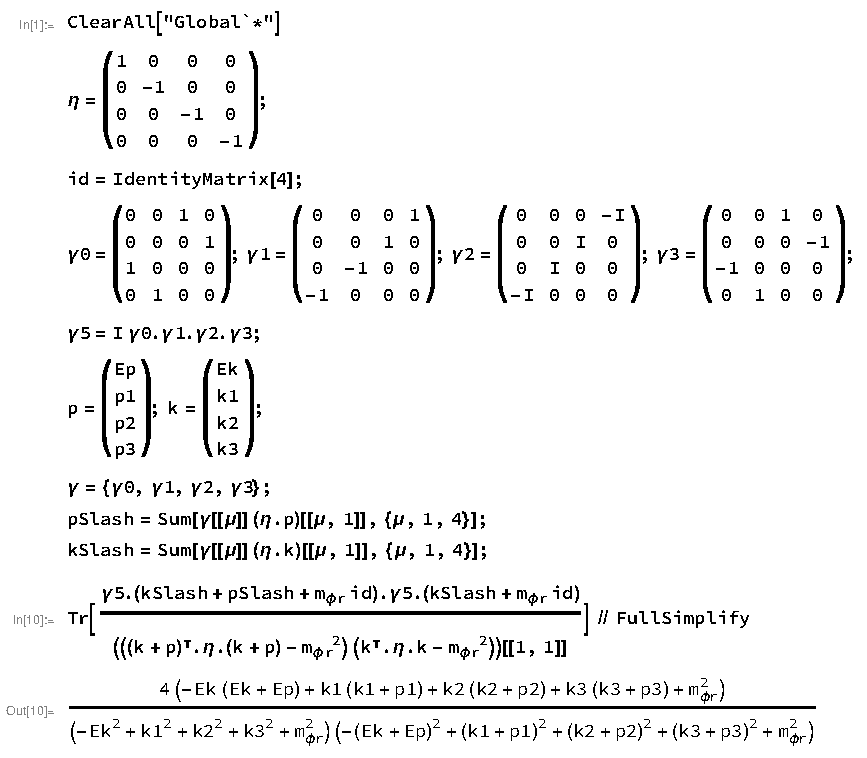
\includegraphics[width=0.9\textwidth]{trace_calculation.pdf}
	}
	\caption{}
	\label{fig:trace_calculation}
\end{figure}{}


We may do likewise for the rest of \cref{eq:phi^4_renormalization_condition,,eq:psi_psibar_renormalization_condition,,eq:phi_psi_psibar_renormalization_condition} to get the rest of the information about the renormalized theory. I do this without showing my calculations.
\begin{align}\label{eq:f_renormalized}
	\feynmandiagram[small, inline=(o.base), horizontal=a to b]{
		o [blob],
		a -- [fermion] o,
		o -- [fermion] b,
	};
	&=
	\feynmandiagram[small, inline=(o1.base), horizontal=a to b]{
		a -- [fermion] o1,
		o1 -- [fermion, half left] o2,
		o2 -- [scalar, half left] o1,
		o2 -- [fermion] b,
	};
	+
	\feynmandiagram[small, inline=(o1.base), horizontal=a to b]{
		o [crossed dot],
		a -- [fermion] o,
		o -- [fermion] b,
	};
	+	\feynmandiagram[small, inline=(o1.base), horizontal=a to b]{
		a -- [fermion] b,
	};. \notag \\
	%
	&= \frac{i g_r^2}{16 \pi^2 (d - 4)} \left( \frac{1}{2} \slashed{p} - m_{\psi_r} \right) + i (\slashed{p} \delta_{Z_\psi} - \delta_{Z_\psi}).
\end{align}
As before, matching powers and using our renormalization conditions, we get
\begin{align}
	\delta_{Z_\psi} &= \frac{- g_r^2}{32 \pi^2 (d - 4)}\\
	%
	\delta_{m_\psi} &= \frac{- g_r^2 m_{\psi_r}}{16 \pi^2 (d - 4)}.
\end{align}
Similarly, expanding \cref{eq:phi_psi_psibar_renormalization_condition}, we get
\begin{align}
	\feynmandiagram[small, inline=(o.base), horizontal=o to a]{
		o [blob],
		o -- [scalar] a,
		o -- [fermion] b,
		c -- [fermion] o,
	};
	&= \frac{-g_r^3}{4 \pi^2 (d - 4)} + \delta_g \gamma^5\\
	%
	\implies \\
	%
	\delta_g &= \frac{g^3}{4 \pi^2 (d - 4)}.
\end{align}
And lastly, 
\begin{align}
	    \feynmandiagram[small, inline=(o.base), vertical=a to b]{
		o [blob],
		a -- [scalar] o,
		b -- [scalar] o,
		a -- [draw=none] b,
		c -- [scalar] o,
		d -- [scalar] o,
		c -- [draw=none] d,
	};
	&= \frac{3 i g_r^4}{4 \pi^2 (d - 4)} + \frac{i \lambda_r^2}{16 \pi^2} - \delta_\lambda\\
	%
	\implies \\
	%
	\delta_\lambda &= \frac{3 i g_r^4}{4 \pi^2 (d - 4)} + \frac{i \lambda_r^2}{16 \pi^2}.
\end{align}


\nocite{*}
\end{document}